\chapter{Results}\label{chap:results}

% TODO: time the training of each model for comparison purposes

\section{Dataset}

We use a dataset from a datacenter of Baidu Inc.
It is a subset of the dataset used in \cite{Zhu13}.

The reason for using only a subset is that due to GDPR limitations we do not have access to the Chinese website where the dataset is hosted.
So, we use a sample from it made available on Kaggle \footnote{\url{https://www.kaggle.com/datasets/drtycoon/hdds-dataset-baidu-inc}}.

Despite only having access to a subset, our dataset includes all the 433 failing disks on the original dataset, which is the most important aspect since in general this is the class with a much smaller amount of members.
It also includes 5317 good disks.

In the dataset, for each disk a sample is taken every hour.
The observation period is of 7 days for good disks and 20 days for bad ones.
In total there are more than a million SMART attribute samples.

The model of every disk is the same.
This model makes available 12 different SMART attributes.
In the dataset they are already normalized to be between -1 and 1.
When including the change rates we compute we can therefore have up to 24 different features for each sample.

\section{Binary Models}

We first perform the experiments using the classical of binary classification, that is of using only two health status levels.
The parameters for these experiments are specified on Appendix \ref{chap:config_files}.
The results for each model is listed on Table \ref{table:results_binary}.

\begin{table}
  \begin{center}
    \begin{tabular}{|c|c|c|c|c|}
      \hline
    Model & FAR(\%) & FDR(\%) & TIA(h) & TIA SD(h) \\
    \hline
    BPNN & 1.69 & 98.46 & 368.5 & 145.8 \\
    RNN & 1.57 & 98.46 & 356.4 & 145.8 \\
    LSTM & 1.50 & 98.46 & 356.7 & 145.6 \\
    Classification Tree & 1.13 & 99.23 & 353.7 & 147.8 \\
    Regression Tree & 0.63 & 99.23 & 348.3 & 147.3 \\
    \hline
    \end{tabular}
    \caption[Results Binary Models]{Results for binary models with standard parameters}
    \label{table:results_binary}
  \end{center}
\end{table}

We also show the distribution of the time in advance with which the failing disks were correctly detected in the histograms of Figures \ref{fig:tia_binary_network} and \ref{fig:tia_binary_tree}.

\begin{figure}
\begin{center}
  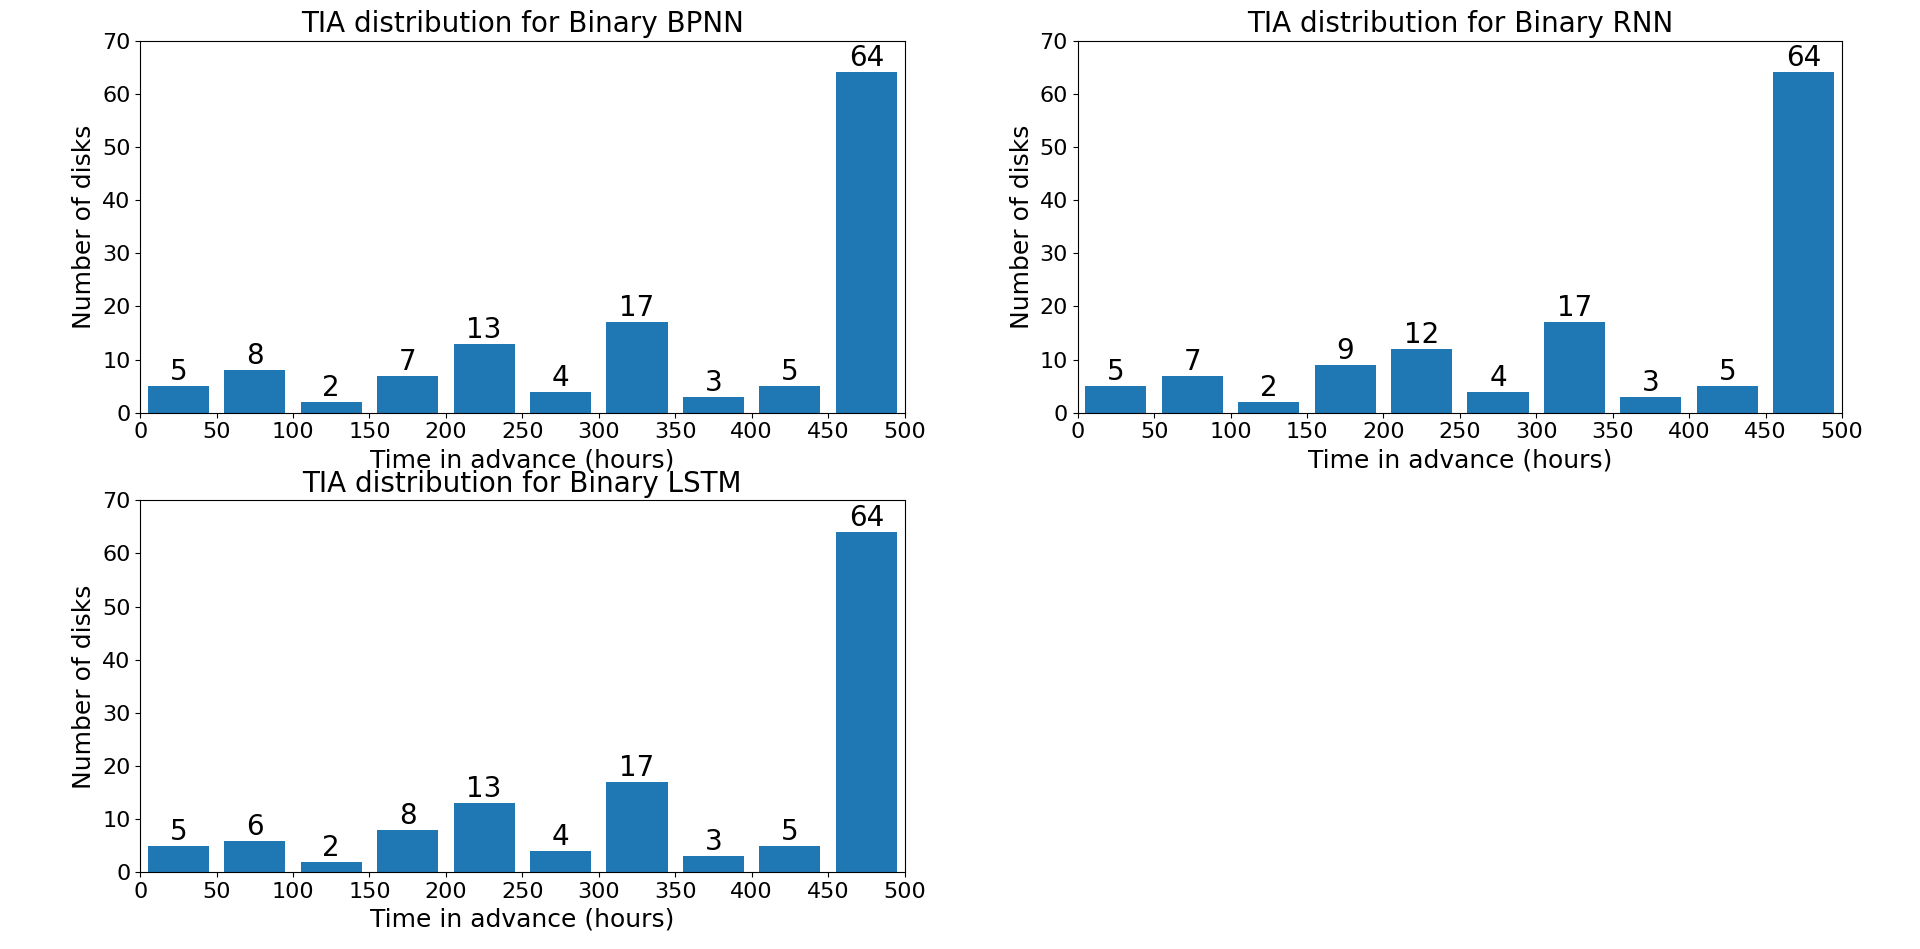
\includegraphics[width=1.0\linewidth]{TIA_Binary_Networks.png}
  \caption[TIA for binary networks]{Time In Advance distribution for binary networks}
  \label{fig:tia_binary_network}
\end{center}
\end{figure}

\begin{figure}
\begin{center}
  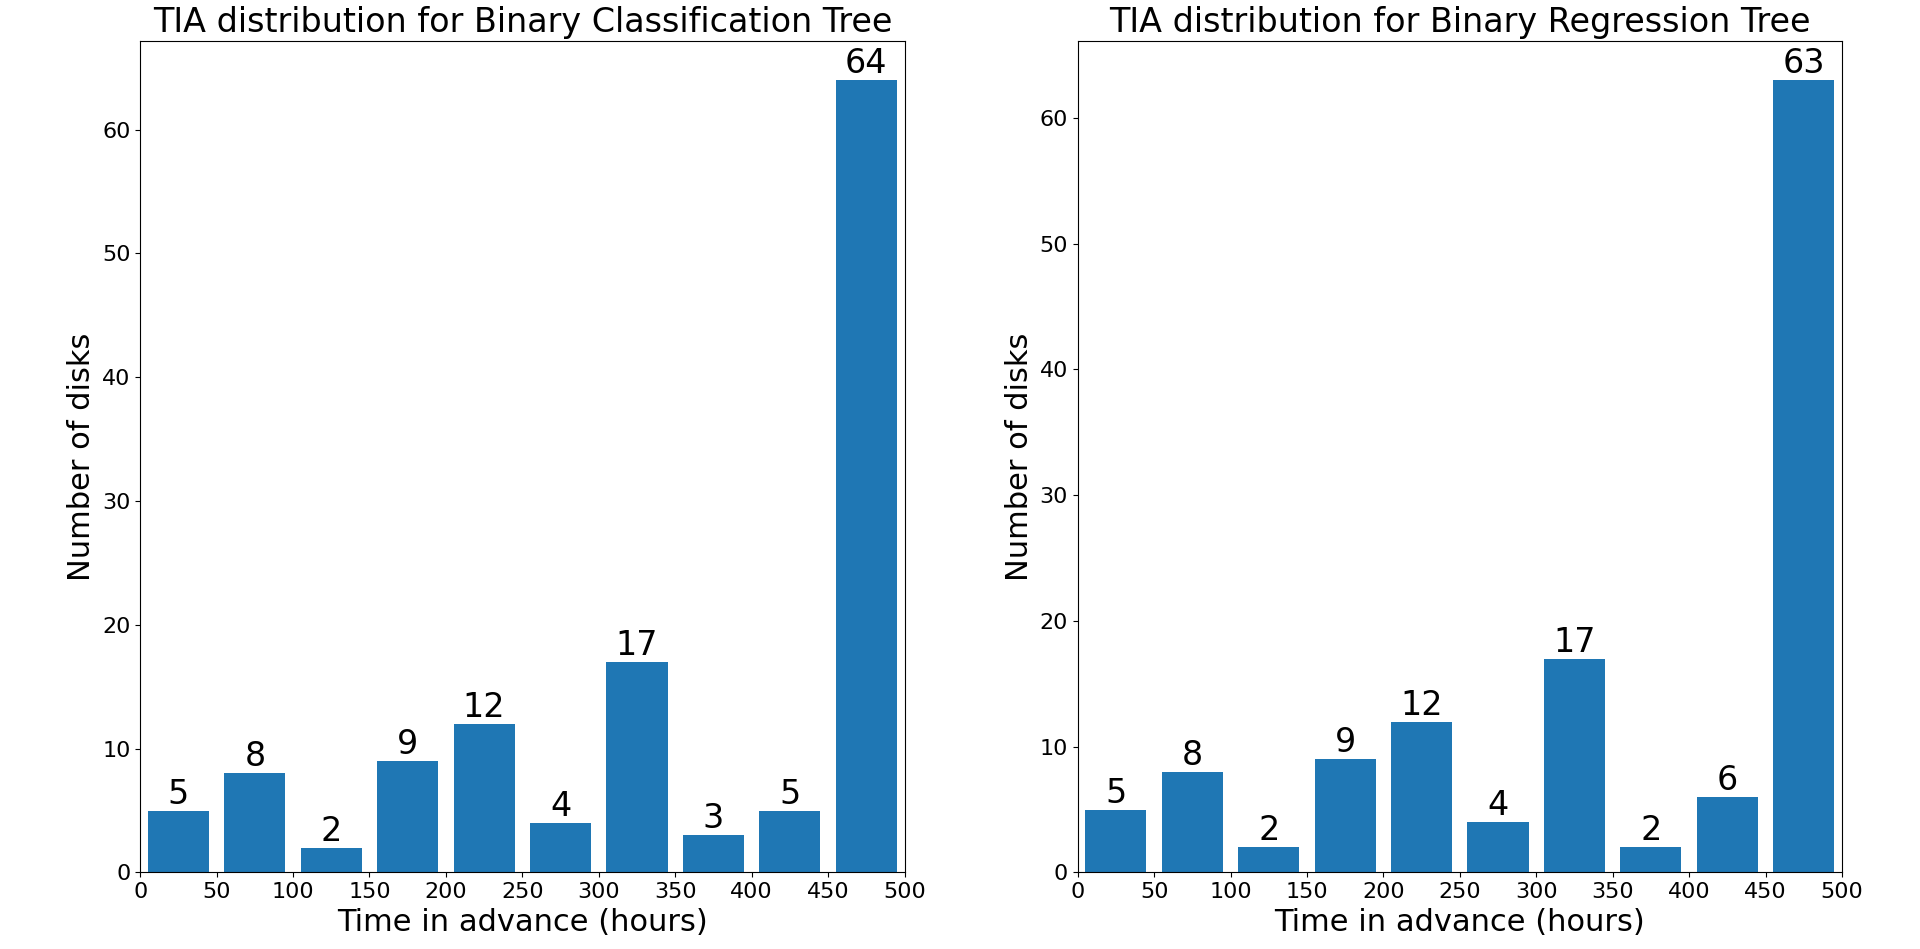
\includegraphics[width=0.9\linewidth]{TIA_Binary_Trees.png}
  \caption[TIA for binary decision trees]{Time In Advance distribution for binary decision trees}
  \label{fig:tia_binary_tree}
\end{center}
\end{figure}

The analysis we can make of these results is firstly that the three network models behave similarly.
LSTM is a little better than the RNN, which is a little better than BPNN.

However, the fact that the three achieve the same FDR indicates that the disks they cannot correctly classify is due more to the nature of the problem than to incorrect hyperparameters.
The cause of these failures that none of the models could predict may be some events that cannot be monitored using SMART attributes such as current surges.

The classification tree performs better than any of the network based models and is only beaten by the regression tree.
This indicates that these older, simpler models are still very powerful and should not be overlooked.

The distribution of the TIA for the different models signals that all of them are capable of detecting signals of problems hundreds of hours in advance
In practical terms, this means that the people responsible for managing the datacenters will have plenty of time to swap the failing disks and prevent any data loss or disruption of service.

The smallest value of the TIA for every model was 19 hours.
This implies that no rushing is needed when a failure is predicted.
The main risk lies instead on the disks that have not been detected.

The capacity of such models to be highly sensitive to failing disks in order to detect problems much before they occur while keeping an FAR below 2\% proves that all of them are powerful methods to tackle the problem at hand.

We can compare our results to other experiments performed on the same dataset in \cite{Zhu13}.
Our results are similar to theirs, who obtained a better FAR of 1.14\% but a slightly worse FDR of 97.69\%.

The advantage of our approach is that we can directly compare the performance of different models without introducing bias due to different datasets or different preprocessing steps.

On the next few pages we will describe the impact of the feature selection algorithms as well as how the voting process can improve the results.
Finally, we will show that the inclusion of the change rates of the SMART attributes improves the performance of every model.

\subsection{Feature Selection Algorithms}

We have trained our different models using the different feature selection algorithms described on Subsection \ref{subsec:feature_selection}.
We still used the default parameters presented on Appendix \ref{chap:config_files}, with the only modifications being on the \verb|feature_count| that was set to 15 and, of course, on \verb|feature_selection_algorithm|.
The results are displayed on Figure \ref{fig:fs_binary}.

\begin{figure}
\begin{center}
  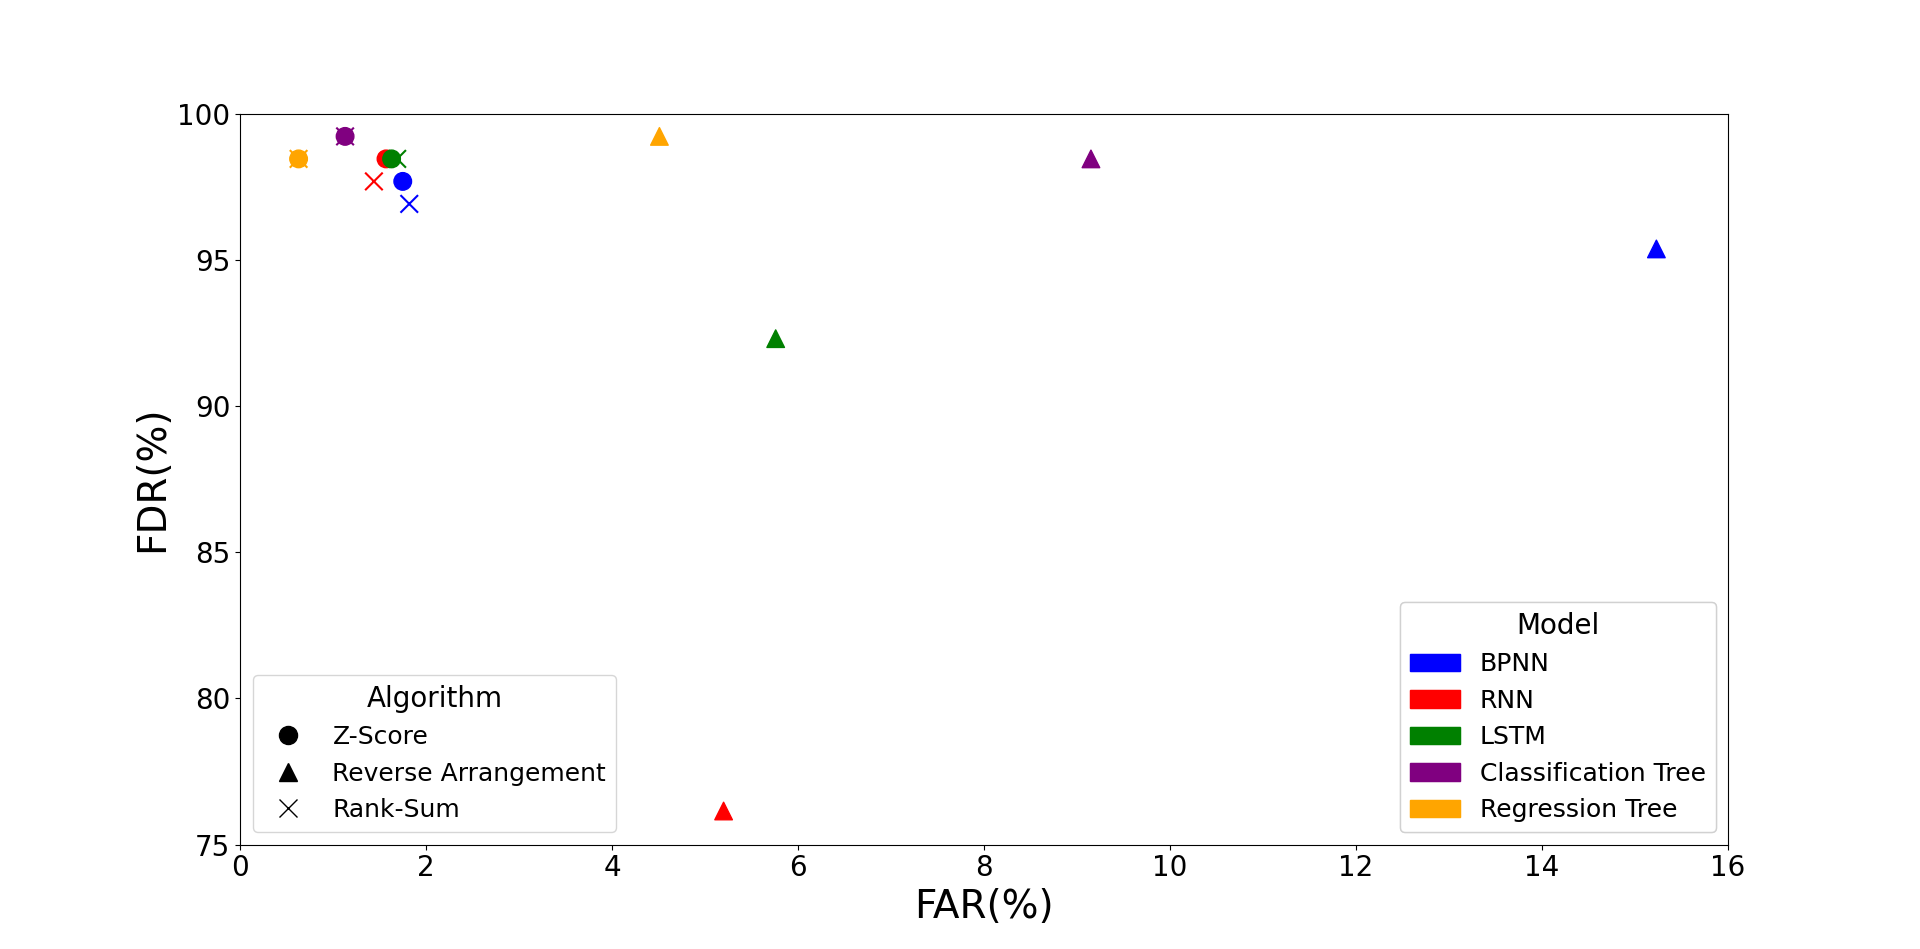
\includegraphics[width=1.0\linewidth]{FS_Binary.png}
  \caption[Feature Selection Results]{Results for different feature selection algorithms for binary models for Feature Count = 15}
  \label{fig:fs_binary}
\end{center}
\end{figure}

The most striking pattern we can observe is that the Reverse Arrangement algorithm had a worse performance than the other two on all scenarios we have tested.

Moreover, the Z-Score algorithm is slightly better than the Rank-Sum test for the network-based models.
However, the result of these two algorithms is the same for our decision trees.

If we observe which features are kept by the three algorithms, we see that 11 of them are common to all of them.
These are features such as Reallocated Sector Count, Temperature and Seek Error Rate, which is to be expected since these can easily indicate failure.

Surprisingly, between the Rank-Sum and the Reverse Arrangement algorithms, only 3 of the 15 features change, but this is already enough to generate completely different results.
Two of the features that appear in the selection done by the Reverse Arrangement but do not appear on Rank-Sum one are change rate features: the Current Pending Sector Change Rate and the Seek Error Rate Change Rate.
The third one, High Fly Writes, also do not appear in the Z-Score selection.

This indicates that the change rate features allow the models to learn the classification problem more efficiently.
We will explore this further on Subsection \ref{subsec:change_rate_impact}.

\subsection{Voting}

To observe how the voting process can influence the performance of the models, we ran our experiments with the default configuration but using 7 votes instead of only 1.
We still kept the vote threshold at 0.5.
As discussed on Subsection \ref{subsec:voting}, for the binary models we are presenting, only the Class Based Voting Algorithm can be used.

The results of this experiment are displayed on Table \ref{table:results_binary_voting}. 

\begin{table}
  \begin{center}
    \begin{tabular}{|c|c|c|c|c|}
      \hline
    Model & FAR(\%) & FDR(\%) & TIA(h) & TIA SD(h) \\
    \hline
    BPNN & 1.69 & 98.46 & 362.7 & 145.6 \\
    RNN & 1.50 & 98.46 & 362.5 & 145.8 \\
    LSTM & 1.50 & 98.46 & 361.3 & 146.2 \\
    Classification Tree & 0.94 & 99.23 & 353.7 & 147.8 \\
    Regression Tree & 0.63 & 98.46 & 353.3 & 148.2 \\
    \hline
    \end{tabular}
    \caption[Results Binary Models with Voting]{Results for binary models with Vote Count set to 7}
    \label{table:results_binary_voting}
  \end{center}
\end{table}

As we can see, the results are very similar to the original ones.
For the RNN model, there was a slight decrease on the FAR.
For the Regression Tree, the FDR decreased a bit and became equal to the ones for the network based models.

Moreover, on all models the TIA decreased a little bit.
This was expected due to the fact that now more than one sample is not enough to classify a disk as failing.

The fact that the FDR didn't change a lot was to be expected given the results displayed on Figures \ref{fig:tia_binary_network} and \ref{fig:tia_binary_tree}.
Usually, a failing disk will start producing samples indicating it much before it crashes.

Therefore, the probability that a sequence with many samples that can be predicted as failing is high.
Thus, the decrease of the FDR is expected to be small, which is the result we obtained.

Now, if we keep the vote count to 7 but increase the vote threshold to 0.8, we obtain the results shown on Table \ref{table:results_binary_threshold}.

\begin{table}
  \begin{center}
    \begin{tabular}{|c|c|c|c|c|}
      \hline
    Model & FAR(\%) & FDR(\%) & TIA(h) & TIA SD(h) \\
    \hline
    BPNN & 1.69 & 98.46 & 362.5 & 145.5 \\
    RNN & 1.38 & 98.46 & 362.3 & 145.4 \\
    LSTM & 0.75 & 98.46 & 362.7 & 145.6 \\
    Classification Tree & 0.94 & 99.23 & 352.3 & 147.6 \\
    Regression Tree & 0.56 & 97.69 & 351.1 & 147.9 \\
    \hline
    \end{tabular}
    \caption[Results Binary Models with Voting]{Results for binary models with Vote Count set to 7}
    \label{table:results_binary_threshold}
  \end{center}
\end{table}

Again we observe a further decrease on the value of the FAR, the FDR and the TIA for some models.
The Regression Tree is able to achieve an FAR as small as 0.56\% which is the smallest value we found for it.

The most interesting approach of using a voting algorithm is that the value of the vote count and threshold can be modified without needing to retrain the model, which is not the case when changing the feature count or the feature selection algorithm.
Therefore, voting is a powerful and fast to use tool to fine tune the FAR-FDR trade off.

\subsection{Change Rate Impact}\label{subsec:change_rate_impact}

The next step was to observe how including the change rate of the original SMART attributes affects the performance of our models.
So, we trained our models without computing the change rates.
In order to remove any impact due to feature selection algorithms, we used all 12 SMART attributes.

The results are displayed on table \ref{table:results_binary_no_change_rate}

\begin{table}
  \begin{center}
    \begin{tabular}{|c|c|c|c|c|}
      \hline
    Model & FAR(\%) & FDR(\%) & TIA(h) & TIA SD(h) \\
    \hline
    BPNN & 2.13 & 98.46 & 363.7 & 145.1 \\
    RNN & 1.57 & 98.46 & 357.4 & 145.9 \\
    LSTM & 2.07 & 95.38 & 361.8 & 143.6 \\
    Classification Tree & 1.07 & 99.23 & 354.7 & 147.8 \\
    Regression Tree & 1.07 & 97.69 & 354.7 & 147.8 \\
    \hline
    \end{tabular}
    \caption[Results Binary Models with Voting]{Results for binary models with Vote Count set to 7}
    \label{table:results_binary_no_change_rate}
  \end{center}
\end{table}

Most notably, every model had a worse performance compared to the original version using the change rates.
This shows that the change rate we computed carries information than can be used by the models to better learn the problem.

Moreover, it is interesting to see that the models that had the best performance were the two Decision Tree ones with information about the change rates.
The fact that they both Classification and Regression Trees are time insensitive implies that we can encode useful information about the problem in the form of change rates. 